\documentclass[conference]{IEEEtran}

\usepackage{graphicx}
\usepackage{cite}
\usepackage{hyperref}
\usepackage{amssymb}
\usepackage{amsmath}
\usepackage{color}
\hyphenation{}
\usepackage[utf8]{inputenc}
\usepackage[ngerman]{babel}


\IEEEoverridecommandlockouts

\title{Praktikumsdokumentation: \\Extraktion von nichtdeterministischen Streaming-String-Transducern aus einem bilingualen Korpus}

\author{\IEEEauthorblockN{Student: \\Alexander Jenke}
\and
\IEEEauthorblockN{Betreuer: \\Thomas Ruprecht, M. Sc.}
\and
\IEEEauthorblockN{Verantwortlicher Hochschullehrer: \\Prof. Dr.-Ing. habil. Heiko Vogler}
}

\begin{document}
\maketitle
\begin{abstract}
\textcolor{red}{TODO}

Der entwickelte Code ist auf \hyperlink{https://github.com/AlexanderJenke/nsst}{GitHub} veröffentlicht.
\end{abstract}

\IEEEpeerreviewmaketitle

\section{Motivation}
\textcolor{red}{TODO\\ ist eine Motivation sinnvoll/notwendig, oder ist es besser direkt mit der Aufgabenstellung zu beginnen?}

\section{Aufgabenstellung}
Ziel des Praktikums ist die Extraktion eines gewichteten nichtdeterministischen Streaming-String-Transducer (NSST) aus einem bilingualen Korpus.
Hierfür sind in der Aufgabenstellung folgende Aufgabenteile definiert:

\begin{itemize}
    \item[1.] Vorbereiten eines bilingualen Europarl-Korpus zur Weiterverarbeitung, wobei nicht zur Sprache gehörende Artefakte entfernt sowie Wörter und Satzzeichen in Token aufgeteilt werden sollen.
    \item[2.] Trainieren eines Hidden-Markov-Model (HMM) auf die Quellsprache und anschließende Extraktion eines endlichen Automaten, welcher die Sprache erkennt.
    \item[3.] Generieren eines totalen Alignments mittels einer geeigneten Methode
    \item[4.] Extraktion und lesbares Speichern der NSST-Regeln mittels Korpus, endlichem Automaten und Alignments
\end{itemize}

\section{Übersicht}
\begin{figure*}
  \center
  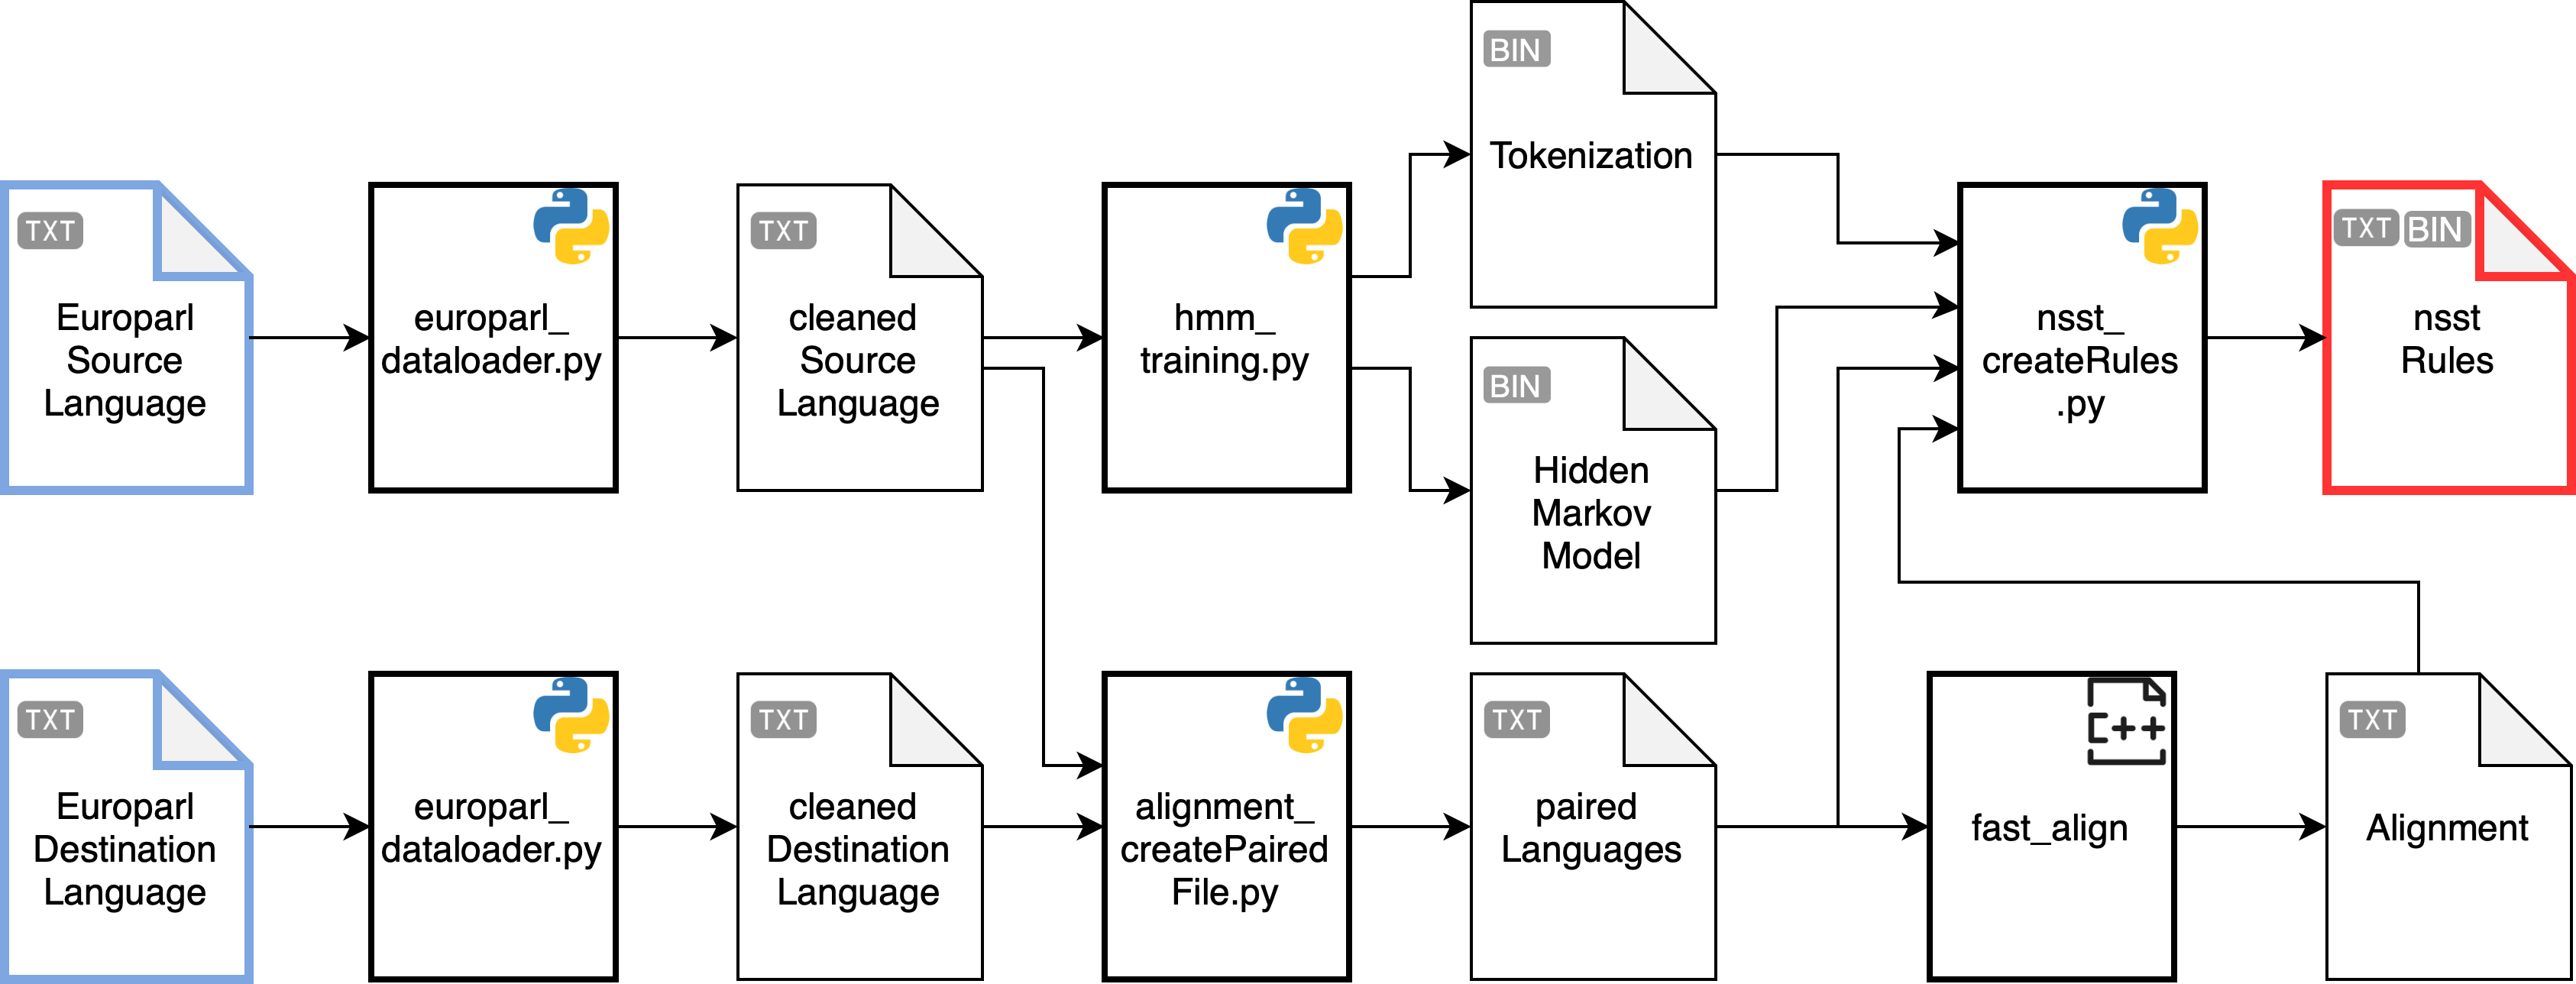
\includegraphics[width=1\textwidth]{img/overview.png}
  \caption{Datenfluss durch die einzelnen Verarbeitungsschritte.}
  \label{Fig:Overview}
\end{figure*}

Die einzelnen Teilschritte wurden in getrennten Skripten implementiert, da einzelne Verarbeitungsschritte rechenaufwendig und zeitintensiv sind.
Zwischenergebnisse werden in separaten Dateien gespeichert, um diese in verschiedenen Experimenten wiederholt nutzen zu können.

Die Aufgabenteile 1,2 und 4 sind vollständig in Python3 implementiert, für Schritt 3 werden die Sprachdaten mit Python3\- vorbereitet und die Alignments mit einer fertigen C++-Implementierung des fast\_align-Algorithmus \cite{fast_align} generiert.

Wie in Abbildung \ref{Fig:Overview} dargestellt, werden die von Europarl bezogenen Sprachdaten durch das \textit{europarl\_dataloader.py}-Skript entsprechend Aufgabenteil 1 vorbereitet, hierbei werden die Datensätze der Quell- und der Zielsprache unabhängig voneinander verarbeitet.
Anschließend wird auf den aufbereiteten Europarldaten der Quellsprache mit dem \textit{hmm\_trainings-py}-Skript ein multinomiales Hidden Markov Model trainiert.
Parallel werden durch das \textit{alignment\_createPairedFile.py}-Skript beide aufbereiteten Sprachdatensätzen in einer Datei kombiniert, aus welcher anschließend mittels dem \textit{fast\_align}-Algorithmus Alignments extrahiert werden.
Abschließend werden das trainierte HMM, die dabei verwendet Zuordnung von Wörtern und Satzzeichen auf Token (Tokenization), die kombinierte Datei beider Sprachdatensätze sowie die generierten Alignments durch das \textit{nsst\_createRules.py}-Skript kombiniert, um die Regeln eines NSST zu erzeugen.

\section{Europarl-Korpus}
\label{Europarl-Korpus}
Grundlage für Extraktion der NSST-Regeln bildet ein bilingualer Sprachdatensatz des Europarl-Korpus der Version 7.
Dieser in \cite{europarl} vorgestellte Korpus enthält bilinguale Daten\-sätze wurden aus den Protokollen der Tagungen des Europäischen Parlamentes extrahiert.
Diese Protokolle sind in 11 Sprachen verfügbar und 20 der 110 möglichen Datensätze sind veröffentlicht.
Die Protokolle im Zeitraum von April 1996 bis November 2011 wurden Blockweise aneinander ausgerichtet und in einzelne Sätze zerlegt. 
Daraus sind Satz-Parallele bilinguale Datensätze mit rund 60 Millionen Wörtern pro Sprache generiert worden \cite{europarl:url}.

Ein bilingualer Datensatz besteht aus zwei Textdateien, welche überwiegend einen Satz pro Zeile enthalten. 
Die Sätze beider Dateien sind anhand der Zeilennummer einander zugeordnet.

\subsection{Sprachauswahl}
Für die Bearbeitung des Praktikums wurde der deutsch-englische Korpus gewählt, um Zwischenergebnisse bewerten zu können, ohne Hilfe durch externe Übersetzungen zu benötigen.
Hierbei ist deutsch als Quell- und englisch als Zielsprache ausgewählt worden.
Da das in Teilaufgabe 2 trainierte HMM ausschließlich auf der Quellsprache trainiert wurde, beeinflusste ebenfalls die einfache Bewertbarkeit der Zwischenergebnisse diese Aufteilung in Quell- und Zielsprache.
Unabhängig davon ist die Implementierung für eine Anwendbarkeit auf alle bilingualen Korpora konzipiert.

\subsection{Aufbereitung}
Entsprechend Teilaufgabe 1 werden die Europarl-Datensätze durch Ausführung des \textit{europarl\_dataloader.py}-Skripts zur Weiterverarbeitung vorbereitet.
Hierfür lädt das Skript jeden Zeile der im Aufruf übergebenen Textdatei und bereinigt diese von allen Zeichen welche nicht explizit erwünscht sind. \\
Explizit erwünschte Zeichen sind:
\begin{itemize}
    \item Buchstaben des Alphabets in Groß- und Kleinschreibung
    \item Umlaute in Groß- und Kleinschreibung, sowie ß
    \item französische Akzente (\`{\space}, \'{\space}, \^{\space}) auf Vokalen in Groß- und Kleinschreibung
    \item Satzzeichen: Punkt, Komma, Ausrufe- und Fragezeichen
    \item Klammern: rund, geschweift und eckig
    \item Schrägstrich, umgedrehter Schrägstrich und Bindestriche
    \item Leerzeichen und Zeilenumbruch
\end{itemize}
Außerdem werden Verschiedene Bindestriche vereinheitlicht und Satzzeichen durch Leerzeichen von Wörtern oder anderen Satzzeichen abgegrenzt, um sicherzustellen, dass diese als einzelne Satzelemente erkannt werden.
Abschließend werden alle aufeinander folgenden Leerzeichen auf ein Leerzeichen reduziert.
Für die spätere Verwendung werden die aufbereiteten Zeilen in einer neuen Textdatei zwischengespeichert.
Die Menge an Wörtern, Satzzeichen, Klammern und Schrägstrichen wird im Folgenden zusammenfassend Vokabeln genannt.

\subsection{Tokenisierung}
Wird das \textit{europarl\_dataloader.py}-Skript von einem anderen Skript eingebunden, stellt es neben der durch das Skript selbst genutzten Funktionalität zur Bereinigung der Sprache auch alle benötigten Funktionen zur Tokenisierung zur Verfügung.

Diese Funktionen werden durch das \textit{hmm\_training.py}-Skript benutzt, um die Vokabeln der aufbereiteten Quellsprache auf maschinenlesbare Tokens zu mappen.
Diese maschinenlesbaren Tokens werden durch nicht-negative Integer-Zahlenwerte repräsentiert.
Für die Erstellung eines Mappings werden unter Beachtung der Groß- und Kleinschreibung die jeweiligen Vorkommen der Vokabeln im verwendeten Datensatz gezählt.
Anschließend werden die Vokabeln der Häufigkeit nach absteigend sortiert und mit 1 beginnend durchnummeriert.
Abweichend davon kann ein Grenzwert festgelegt werden, ab welchem Vokabeln dem Sammel-Token mit der Nummer 0 zugewiesen werden, sobald deren Häufigkeit dem Grenzwert gleichen oder diesen unterschreiten.
Die daraus resultierende Funktion ist surjektiv und wird im Folgenden Tokenisierung genannt.
Wird kein Grenzwert definiert, ist die Tokenisierung bijektiv.

\section{Hidden-Markov-Model}
Entsprechend Teilaufgabe 2 wird durch Ausführen des \textit{hmm\_training.py}-Skripts ein Hidden Markov Model unsupervised auf der Quellsprache trainiert.
Das HMM kann als 5-Tupel definiert werden \cite{hmm->wfsm}:
\begin{equation}\notag
\begin{aligned}
HMM &= (Q, \Sigma, I, T, E) && \text{, mit} \\
Q &= \{ q_0, q_1, ...\} \\
\Sigma &= \{0,1,...\} \\
I &= Q \rightarrow \mathbb{R}^+ \\
T &= Q \times Q \rightarrow \mathbb{R}^+ \\
E &= Q \times \Sigma \rightarrow \mathbb{R}^+ \\
\end{aligned}
\end{equation}
Hierbei ist $Q$ die Menge der Zustände, $\Sigma$ die Menge der Token (Alphabet), $I$ die Startwahrscheinlichkeit der Zustände, $T$ die Übergangswahrscheinlichkeit von einem Zustand zum nächsten und $E$ die Emissionswahrscheinlichkeit eines Token in einem Zustand \cite{hmm->wfsm}.

Für das Training werden die Funktionen $S$, $T$ und $E$ des HMMs zufällig initialisiert und anschließend in mehreren Iterationen durch einen EM-Algorithmus auf die Sätze des Trainingsdatensatzes angepasst \cite{hmmTraining}.

\subsection{Architektur}
Das HMM ist mittels der \textit{MultinomialHMM}-Klasse des hmmlearn-Packages \cite{hmmlearn} implementiert. 
Dieser HMM-Typ emittiert in jedem Zustand entsprechend einer Gewichtung einen Token.
Es kann von jedem Zustand entsprechend einer Probabilistik in jeden Zustand gewechselt werden.
Die Anzahl der Zustände und Token kann bei der Initialisierung beliebig gewählt werden.\\
Sei $n_s$ die Anzahl der Zustände und $n_t$ die Anzahl der Token, dann wird das HMM durch folgende drei Matrizen vollständig beschrieben:
\begin{description}
\item[startprob]\hfill \\
Die $1\times n_s$-Matrix definiert die \\Startwahrscheinlichkeiten $I$ der Zustände.\\
\item[transprob]\hfill \\
Die $n_s\times n_s$-Matrix definiert die \\Übergangswahrscheinlichkeiten $T$ zwischen \\Zuständen.\\
\item[emissionprob]\hfill \\
Die $n_s\times n_t$-Matrix definiert die \\Emissionswahrscheinlichkeiten $E$ der Token.
\end{description}
Zustände und Token sind durch nicht-negative Integer-Werte repräsentiert und lassen sich somit direkt als Index auf die Matrizen anwenden.

Um das Training zu beschleunigen, wurde eine MultiThreading Variante des MultinomialHMM implementiert.
Diese berechnet im E-Schritt des EM-Algorithmus in mehreren Threads parallel die logarithmische Wahrscheinlichkeit der einzelnen Sätze des Trainingsdatensatzes.
Lediglich das Akkumulieren der für den M-Schritt benötigten Statistiken wird hierbei Sequenziell ausgeführt.
Hierdurch wird die Rechenzeit bei Verdopplung der Threads nahezu halbiert, solange die Anzahl echter Kerne nicht überschritten wird.

\subsection{Hyperparameter}
Ausschlaggebend für den Erfolg beim Training des HMM ist die Wahl der Hyperparameter.
Im Folgenden werden die zu wählenden Parameter sowie eventuelle Kriterien erläutert.

Die \textbf{train\_step\_size (TSS)} definiert in welcher Schrittgröße über die Sätze des Datensatzes gelaufen wird. 
Grundsätzlich sind die ersten 4096 Sätze der Evaluation des Modells vorbehalten, diese Sätze bilden den Testdatensatz. 
Alle verbleibenden Sätze können für das Training verwendet werden, jedoch kann die Größe dieses Datensatzes reduziert werden, indem nur jeder TSS-te Satz verwendet wird. 
Ausschlaggebend für die Wahl des TSS ist die Abwägung zwischen Speicher- und Rechenaufwand gegenüber einer ausreichenden Größe für einen repräsentativen Datensatz. 
Standardmäßig ist dieser Wert mit 20 implementiert.
Der daraus resultierende Datensatz umfasst 95.806 Sätze mit 2.518.714 Vokabeln und 84.102 Token.

Der in Kapitel \ref{Europarl-Korpus} erläuterte \textbf{Threshold} reduziert die Anzahl der Token, indem seltene Vokabeln im kumulativen Token 0 zusammenfasst werden.
Dieser Parameter ist mit einem Standardwert von 4 implementiert, da bei stichprobenartiger Auswertung auf dem verwendeten deutschen Korpus bis zu diesem Wert überwiegend Eigennamen sowie viele Verben in konjugierter Form vorgekommen sind. 
Ab einem Wert von 5 wären vermehrt Verben in Grundform sowie beschreibende Vokabeln betroffen.
Hierdurch reduziert sich die Zahl der Token auf 19.440.
Somit werden 76,89\% der möglichen Token im kumulativen Token 0 zusammengefasst, jedoch wirkt sich diese Reduktion nur auf 96044 Vokabelvorkommen aus, lediglich 3,81\% der gesamten Trainingsdaten. 
Diese Werte beziehen sich auf einen TSS von 20, eine Übersicht über die Auswirkung verschiedener Threshold-Werte und weitere TSS ist im Anhang zu finden.

Während sich die Anzahlt der Token aus dem Datensatz ergeben, muss die \textbf{Anzahl der Zustände} des HMM festgelegt werden. 
Da dieser Wert die Größe des HMM bestimmt, sollte er mit Bedacht gewählt werden.
Pro Zustand entwickeln sich während dem Training verschiedene Emissionswahrscheinlichkeiten der Token, wodurch semantisch und syntaktisch korrekte Sätze eine höhere Wahrscheinlichkeit erreichen.
Da die Zustände somit indirekt die Kontext-Information des bisherigen Satzes abbilden, muss deren Anzahl ausreichen, um die Komplexität der Quellsprache abzubilden.
Eine Obergrenze wird durch die zu trainierenden freien Parameter und die Zahl der Datenpunkte in den Trainingsdaten gebildet.
Sei $n_s$ die Anzahl der Zustände und $n_t$ die Anzahl der Token, so lässt sich die Anzahl freier Parameter $n_param$ wie folgt berechnen:
\begin{equation}\notag
n_{param} = (n_s-1) + [n_s * (n_s-1)] + [n_s * (n_t-1)]
\end{equation}
Hierbei ergibt sich der erste Summand aus den Startwahrscheinlichkeiten $I$. Da diese aufsummiert eins ergeben, lässt sich der letzte Wert aus allen vorherigen bestimmen, und es bleiben $(n_s-1)$ freie Parameter.\\
Der zweite Summand ergibt sich aus den Transitionswahrscheinlichkeiten $T$.
Pro Zustand summieren sich die Übergangswahrscheinlichkeiten zum nächsten Zustand ebenfalls zu eins auf.
Somit bleiben für jeden Zustand $(n_s-1)$ freie Parameter, also gesamt $[n_s * (n_s-1)]$.\\
Der dritte Summand ergibt sich aus den Emissionswahrscheinlichkeiten $E$.
Pro Zustand Summieren sich die Wahrscheinlichkeiten aller Token zu eins auf und es bleiben $[n_s * (n_t-1)]$ freie Parameter.\\
Ist die Anzahl der freien Parameter größer als die Zahl der Datenpunkte, können nicht alle Parameter bestimmt werden und die Lösung ist degeneriert \cite{degenerate}.
Somit führt eine größere Anzahl an Zuständen ab diesem Punkt lediglich zu einen höheren Rechenaufwand ohne neue Informationen in den Zuständen abzubilden.\\
Die Anzahl der Datenpunkte im Datensatz entspricht der Anzahl der Vokabeln.
Ein TSS von 20 führt zu 2.518.581 Vokabeln, ein Threshold von 4 zu 19440 Token. 
Damit liegt für diese Parameter die Obergrenze der Zustände bei 128. \\
In der Implementierung wurde das HMM mit 10, 54, 100 und 200 Zuständen trainiert.
Hierbei entsprechen die 54 Zustände den in \cite{germanCorpus} definierten 54 POS-Tags.
Mit steigender Anzahl an Zuständen, hat sich beim Training eine steigende Wahrscheinlichkeit der Test- und Trainingsdaten gezeigt, jedoch ist auch die Berechnungszeit gestiegen.
Somit muss bei der Wahl dieses Parameters, unter Beachtung der erläuterten Grenzen, zwischen guter Repräsentation des Datensatzes und Rechenaufwand abgewogen werden.

Abschließend muss für das Training noch bestimmt werden, in wie vielen \textbf{Iterationen} das HMM auf den Datensatz angepasst werden soll. 
In jeder Iteration wird der komplette Datensatz im E-Schritt des EM-Algorithmus verarbeitet und anschließend das HMM im M-Schritt angepasst.
Da die Anpassungen in kleinen Schritten erfolgt wird eine ausreichende Anzahl an Iterationen benötigt um gute Ergebnisse zu erzielen.
Jedoch kann es bei zu vielen Schritten zu einer übermäßigen Anpassung (Overfitting) auf die Trainingsdaten kommen, sodass das Model an Allgemeingültigkeit verliert.
Dies wird in einer fallenden Wahrscheinlichkeit der Testdaten bei steigender Wahrscheinlichkeit der Trainingsdaten deutlich.
In der Implementierung haben sich 100 Iterationen bewährt, da zu diesem Zeitpunkt die Wahrscheinlichkeiten nicht mehr stark stiegen und es noch nicht zu Overfitting kam. 

\subsection{endlicher Automat}
Wie in\cite{hmm->wfsm} beschreiben wird, kann aus einem HMM ein Automat abgeleitet werden, welcher die Quellsprache erkennt.
Hierfür wird der gewichteter endlicher Automat (WFSA) wie folgt definiert:
\begin{equation}\notag
    \begin{aligned}
        HMM &= (Q, \Sigma, I, T, E) \\
        WFSA &= (Q_A, \Sigma_A, \delta_A, I_A, P_A, F_A) \\
        Q_A &= Q \cup \{q_{-1}\} \\
        \Sigma_A &= \Sigma \\
        \delta_A &=\{(q_{-1}, a, q) \colon I(q) \not= 0\land E(q,a) \not= 0\} \\
        \delta_A &=\{(q', a, q) \colon T(q', q) \not= 0\land E(q,a) \not= 0\} \\
        I_A(q_{-1}) &= 1 \\
        I_A(q) &= 0 \\
        P_A(q_{-1}, a, q) &= I(q) \cdot E(q, a)\\
        P_A(q', a, q) &= T(q', q) \cdot E(q, a)\\
        F_A(q_{-1}) &= 0 \\
        F_A(q) &= 1 \\
        &\text{wobei } \forall q,q'\in Q,a\in \Sigma\\
    \end{aligned}
\end{equation}
Hierbei ist $Q_A$ die Menge der Zustände des HMM, erweitert um den Startzustand $q_{-1}$.
Das Alphabet $\Sigma_A$ gleicht dem HMM.
Die Übergänge $\delta_A$ lesen ein Zeichen aus dem Alphabet und verbinden Zustände deren Transitionswahrscheinlichkeit $T$ im HMM nicht 0 ist, sowie den Startzustand mit allen Zuständen deren Startwahrscheinlichkeit $I$ nicht 0 ist.
Die Anfangsgewichte $I_A$ definieren den Startzustand als einzig möglichen Anfangszustand, die Endgewichte $F_A$ definieren alle Zustände außer den Startzustand als Finalzustände.
Die Übergangsgewichte $P_A$ sind das Produkt aus der Transitionswahrscheinlichkeit $T$ mit der Emissionswahrscheinlichkeit $E$ des gelesenen Tokens im Zielzustand, wobei die Transitionswahrscheinlichkeit vom Startzustand zu einem anderen Zustand der Startwahrscheinlichkeit $I$ entspricht. Zu beachten ist, dass hierbei die Übergangsgewichte eine Probabilität der Nutzung dieser Kante angeben, für eine Interpretation als Kosten müssen die Werte von eins subtrahiert werden. 

Der resultierende Automat kann bei der NSST-Regel-Extraktion eine Zustandsreihenfolge für die Verarbeitung des Quell-Satzes bereitstellen.
Alternativ dazu kann direkt mit dem HMM die ideale Zustandsfolge für den zu übersetzenden Satz ermittelt werden.

\section{Alignment}
Die Alignments verbinden die Vokabeln der Quell- und Zielsätze entsprechend ihrer semantischen Korrelation und geben somit Auskunft, welche Vokabel im Quellsatz, welche Vokabeln des Zielsatzes erzeugt. 
Für eine Übersetzung muss jede Vokabel des Zielsatzes von genau einer Vokabel des Quellsatzes erzeugt werden, diese Eigenschaft heißt total. \\
Sei $X$ die Menge aller Vokabeln des Quellsatzes und $Y$ die Menge aller Vokabeln des Zielsatzes, dann ist die Funktion $f(x) = y, \exists! x \in X, \forall y \in Y $ ein totales Alignment. 

Diese totalen Alignments werden mittels des \textit{fast\_align}-Algorithmus \cite{fast_align} generiert.
Dieser passt durch den EM-Algorithmus ein lexikalisches Übersetzungsmodell an die eingegebenen Satzpaare an \cite{fast_align} und gibt am Ende ein Alignment pro Satz aus.
Ein Alignment besteht aus einer Zeile und enthält mehrere Satzpositionspaare welche durch ein Leerzeichen getrennt sind.
Diese Satzpositionspaare enthalten jeweils eine Satzposition der Quell- und Zielsprache, getrennt durch einen Bindestrich.

Die benötigte Eingabedatei wird durch Ausführen des \textit{alignment\_createPairedFile.py}-Skripts generiert und enthält in jeder Zeile den Quell- und Zielsatz, getrennt durch das von \textit{fast\_align} geforderte Trennzeichen \glqq{} $ ||| $ \grqq .

Wird der \textit{fast\_align}-Algorithmus mit den Optionen -d, -o, -v und -N ausgeführt generiert dieser ein totales Alignment.
Hierbei sind die ersten drei Optionen durch die Entwickler ausdrücklich empfohlen und führen zur Verwendung einer Dirichlet-Verteilung und der Bevorzugung von Verknüpfungen nahe der monotonen Diagonale. 
Die N-Option verbietet die Nutzung des null-Wortes und führt zu einem totalen Alignment.
Bei nicht-Benutzung der vierten Option müssen nicht alle Satzpositionen der Zielsprache einem Satzpositionspaar zugeordnet werden.


\section{nichtdeterministischer Streaming-String-Transducer}
Abschließend werden entsprechend Teilaufgabe 4, durch Ausführen des \textit{nsst\_createRules.py}-Skripts, die Regeln des NSST extrahiert.
Hierfür werden das trainierte HMM, die verwendet Tokenization, die kombinierte Datei beider Sprachdatensätze sowie das dazugehörige Alignment verarbeitet und für jeden Satz die zur Übersetzung benötige Menge an Regeln generiert.

\subsection{Span}
Anhand der Alignments wird ermittelt welche Vokabel der Quellsprache welche 
Vokabeln der Zielsprache generiert. 
Für jede Position im Quellsatz lässt sich bestimmen welche Satzpositionen im Zielsatz bereits generiert wurden. 
Diese Funktion welche eine Quellsatzposition auf eine Menge zusammenhängender Zielsatzpositionen abbildet, nennen wir im Folgenden $Span$.
Sei $G$ eine Funktion, die für eine Quellsatzposition die Menge der durch diese Wortposition generierten Zielsatzpositionen gibt, $\{p_0, p_1,..., p_n\}$ die Menge der Quellsatzpositionen und $\{q_0, q_1,..., q_m\}$ die Menge der Zielsatzpositionen, dann lässt sich  $Span$ wie folgt definieren:

\begin{equation}\notag
    \begin{aligned}
        Span(p_i) &= \{Span(p_{i-1}) \cup G(p)\} && \forall p \in \{p_1, p_2, .. , p_n\}\\
        Span(p_0) &= \{G(p_0)\}\\
        Span(p_n) &= \{q_0, q_1, ... , q_m\}
    \end{aligned}
\end{equation}
Die Menge der Zielsatzpositionen einer Quellsatzposition lassen sich in Submengen teilen, sodass jede Submenge alle Positionen zwischen der keinsten und größten enthaltenen Satzposition enthält. Diese Submengen lassen sich durch eben diese kleinste und größte enthaltene Satzposition beschreiben.

\subsection{NSST-Regel}
Eine Regel des NSST ist eine Funktion der Form 
\begin{equation}\notag
    \begin{aligned}
        Rule: Q \times \Sigma_{src} &\times \Sigma_{tgt}^{**} \rightarrow Q \times \Sigma_{tgt}^{**}
    \end{aligned}
\end{equation}
Sie liest einen Zustand $Q$, einen Token der Quellsprache $\Sigma_{src}$ und eine Menge von Mengen von Token der Zielsprache $\Sigma_{tgt}^{**}$ und gibt einen neuen Zustand sowie eine neue Menge von Mengen von Token.
Die Menge von Mengen von Token wird im Folgenden Register genannt.
Die Menge von Mengen im Register ist beliebig aber endlich.
Im Register wird durch Aneinanderreihung von Regeln die Übersetzung des Quellsatzes zusammengesetzt.
Hierfür wird das ausgegebene Register aus den Mengen des eingegebenen Registers und Token der Quellsprache mittels no-copy Operationen zusammengesetzt.
Das heißt, dass eine Menge des eingegebenen Registers maximal einmal im ausgegebenen Register verwendet werden darf.
Sind alle Token des Quellsatzes gelesen, steht in einer definierten Menge des Registers die Übersetzung.
In der Implementierung wird hierfür die erste Menge im Register verwendet.

\subsection{Regel-Extraktion}
Zuerst wird für die Regel-Extraktion eine Zustandsreihenfolge für den Quellsatz ermittelt.
In der Implementierung wird hierfür das Satzpaar tokenisiert und mit dem HMM die wahrscheinlichste Zustandsfolge für den Quellsatz berechnet.
Diese wird um den Anfangszustand $q_{-1}$ ergänzt.
Hierdurch gleicht die Anzahl der Zustandsübergänge der Anzahl der Token des Quellsatzes.
Zum i-ten Zustandsübergang gehört entsprechend der i-te Token des Quellsatzes.
Ein leeres Register wird initialisiert.
Anschließend wird für jeden Zustandsübergang $q_n \rightarrow q_m$ eine Regel generiert, welche:
\begin{itemize}
    \item Den Zustand $q_n$ ließt
    \item Den zugehörigen Token ließt
    \item Den Zustand $q_m$ ausgibt
    \item Im Ausgaberegister den Span der Satzposition des Token erzeugt
\end{itemize}
Der Span der Satzposition wird durch entsprechendes aneinanderreihen der Mengen des eingegebenen Register und den von dieser Position erzeugten Token erzeugt (siehe Beispiel im Anhang).
Das Ausgaberegister wird anschließend als Eingaberegister für die nächste Regel verwendet.
Die erzeugten Regeln werden gesammelt, existiert eine Regel bereits, wird für diese ein Zähler erhöht.
Dieser Zähler wird bei der Übersetzung zur Berechnung der Regelwahrscheinlichkeit verwendet.


\section{Diskussion}
\textcolor{red}{TODO\\
Europarl-Probleme\\
kumulativer Token verbesserbar\\
semantische Validierung der Alignments notwendig\\
'statistische' Analyse der extrahierten Regeln\\
weitere Evaluationsergebnisse ...\\}


% references section
\bibliographystyle{IEEEtran}
\bibliography{P-PnS.bib}

\section{Anhang}
\subsection{Beispiel: Regel-Extraktion}
Gegeben:\\
Quellsatztoken:  1 1 2\\
Zielsatztoken: 3 3 5 4 4\\
Alignment: 0-0 0-3 1-1 1-4 2-2\\
Zustandsfolge: $q_{-1} \rightarrow q_0 \rightarrow q_1 \rightarrow q_2$\\

Extrahierte Regeln:\\
$q_{-1} -1-> q_0$ [3, 4] / 1\\
$q_0 -1-> q_1$ [x0 3, x1 4] / 1\\
$q_1 -2-> q_2$ [x0 5 x1] / 1\\

Hierbei ist eine Regel als \glqq Quellzustand $-$ Token $->$ Zielzustand [Registeroperation] / Zähler\grqq{}  zu lesen.
Einzelne Mengen im Register sind durch ein Komma getrennt.
\glqq x0\grqq{} steht für das Kopieren der ersten Menge des eingegebenen Registers.
Integer ohne vorangestelltes \glqq x\grqq{} sind von dieser Regel erzeugte Token der Zielsprache.
Die einzelnen, durch Leerzeichen getrennten Elemente der Registeroperationen 
werden konkateniert, um den Inhalt der neuen Registermenge zu erzeugen.


\subsection{Tabellen}
\begin{table}[htbp]
    \centering
    \begin{tabular}{|c|c|c|c|c|}
        \hline
        \textit{TSS = 1} & \multicolumn{2}{|c|}{ \textbf{Vokabeln}} & \multicolumn{2}{|c|}{ \textbf{Vokabel-Vorkommen}} \\
        \hline
        \textbf{Threshold} & \# & \% & \# & \% \\
        \hline
        All & 404387 & - & 50220274 & - \\
        1 & 207333 & 51,27 & 207333 & 0,41 \\
        2 & 260282 & 64,36 & 313231 & 0,62 \\
        3 & 286078 & 70,74 & 390619 & 0,78 \\
        4 & 301604 & 74,58 & 452723 & 0,90 \\
        5 & 312604 & 77,30 & 507723 & 1,01 \\
        6 & 320840 & 79,34 & 557139 & 1,11 \\
        7 & 327183 & 80,91 & 601540 & 1,20 \\
        8 & 332410 & 82,20 & 643356 & 1,28 \\
        9 & 336794 & 83,29 & 682812 & 1,36 \\
        10 & 340479 & 84,20 & 719662 & 1,43 \\
        \hline
        \multicolumn{5}{}{}
    \end{tabular}
    \caption{Auswirkung verschiedener Threshold-Werte auf den deutschen Korpus mit TSS=1}
\end{table}

\begin{table}[htbp]
    \centering
    \begin{tabular}{|c|c|c|c|c|}
        \hline
        \textit{TSS = 20} & \multicolumn{2}{|c|}{ \textbf{Vokabeln}} & \multicolumn{2}{|c|}{ \textbf{Vokabel-Vorkommen}} \\
        \hline
        \textbf{Threshold} & \# & \% & \# & \% \\
        \hline
        All & 84102 & - & 2518714 & - \\
        1 & 45184 & 53.73 & 45184 & 1.79 \\
        2 & 56052 & 66,65 & 66920 & 2,66 \\
        3 & 61368 & 72,97 & 82868 & 3,29 \\
        \textbf{4} & \textbf{64662} & \textbf{76,89} & \textbf{96044} & \textbf{3,81} \\
        5 & 66931 & 79,58 & 107389 & 4,26 \\
        6 & 68624 & 81,60 & 117547 & 4,67 \\
        7 & 70001 & 83,23 & 127186 & 5,05 \\
        8 & 71053 & 84,48 & 135602 & 5,38 \\
        9 & 71997 & 85,61 & 144098 & 5,72 \\
        10 & 72752 & 86,50 & 151648 & 6,02 \\
        \hline
        \multicolumn{5}{}{}
    \end{tabular}
    \caption{Auswirkung verschiedener Threshold-Werte auf den deutschen Korpus mit TSS=20}
\end{table}

\end{document}

